\documentclass{article}
\usepackage[T1]{fontenc}
\usepackage[utf8]{inputenc}
\usepackage{amsmath,amssymb}
\usepackage{tikz}
\usepackage{tikzsymbols}
\usetikzlibrary{arrows,automata}
\usepackage{tabularx}
\usepackage{lmodern}
\usepackage{xcolor}
\usepackage{pbox}
\usepackage{algorithm2e}
\usepackage{listings}
\usepackage{titlesec}

\titlelabel{\thetitle. Aufgabe}

\setlength\parindent{0pt}

\begin{document}

\begin{center}
  \Large{Informatik D -- Klausur 2013 -- Nebentermin -- Fisole}

  \large{Sebastian Höffner, Andrea Suckro, Judith Kemper}
\end{center}

\section{}
\begin{enumerate}
	\item Reguläre Sprachen (Typ 3)
	\item Kontextfreie Sprachen (Typ 2)
	\item Rekursiv aufzählbare Sprachen (Typ 0)
\end{enumerate}


\section{}
Alles nach rechts ankreuzen ab\dots
\begin{enumerate}
	\item \dots regulär
  \item \dots rekursiv aufzählbar
  \item \dots regulär ($\emptyset$)
  \item \dots deterministisch kontextfrei
\end{enumerate}

\section{}
\begin{center}
NDEA Zwischenschritt\par
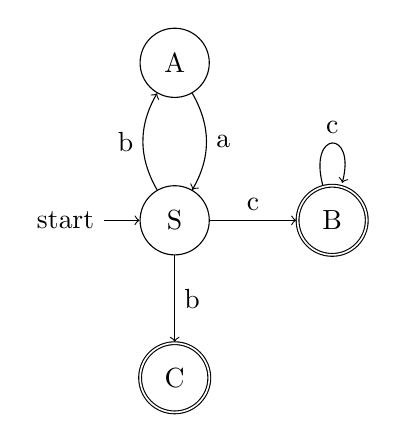
\begin{tikzpicture}[->, auto, node distance=2cm]
	\node[initial,state]   (S) {S};
  \node[state]           (A) [above of = S] {A};
  \node[state,accepting] (B) [right of = S] {B};
  \node[state,accepting] (C) [below of = S] {C};
  \path (S) edge [bend left] node {b} (A)
        (A) edge [bend left] node {a} (S)
        (S) edge [] node {c} (B)
        (B) edge [loop above] node{c} (B)
        (S) edge [] node {b} (C);
\end{tikzpicture}
\end{center}
\begin{align*}
S &\rightarrow bA | cB | bC \\
A &\rightarrow aS \\
B &\rightarrow cB | \epsilon \\
C &\rightarrow \epsilon \\
\end{align*}

Vereinfacht:
\begin{align*}
S &\rightarrow bA | cB | c | b \\
A &\rightarrow aS \\
B &\rightarrow cB | c \\
\end{align*}


\section{}
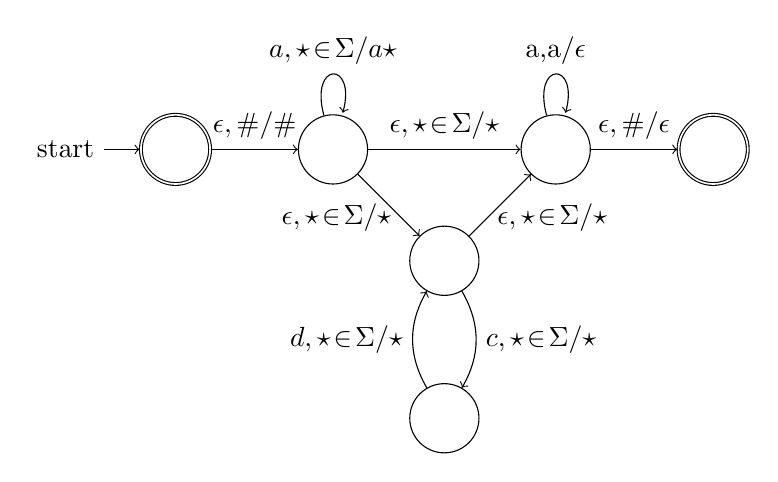
\begin{tikzpicture}[->, auto, node distance=2cm]
	\node[initial,state,accepting]   (A) {};
  \node[state]           (B) [right of = A] {};
  \node[state]           (E) [below right of = B] {};
  \node[state]           (C) [above right of = E] {};
  \node[state,accepting] (D) [right of = C] {};
  \node[state]           (F) [below of = E] {};
  \path (A) edge [] node {$\epsilon,\#/\#$} (B)
        (B) edge [loop above] node {$a,\star\!\in\!\Sigma/a\star$} (B)
            edge [] node {$\epsilon,\star\!\in\!\Sigma/\star$} (C)
            edge [left, pos=0.7] node {$\epsilon,\star\!\in\!\Sigma/\star$} (E)
        (E) edge [bend left] node {$c,\star\!\in\!\Sigma/\star$} (F)
            edge [right, pos=0.3] node {$\epsilon,\star\!\in\!\Sigma/\star$} (C)
        (F) edge [bend left] node {$d,\star\!\in\!\Sigma/\star$} (E)
        (C) edge [] node {$\epsilon,\#/\epsilon$} (D)
            edge [loop above] node {a,a/$\epsilon$} (C);
\end{tikzpicture}


\section{}
Es können Kontextfreie Sprachen dargestellt werden.

Chomskynormalform: $V \rightarrow V \times V$ und $V \rightarrow \Sigma$.

Greibachnormalform: $V \rightarrow \Sigma \times V^*$.



\section{}
\begin{enumerate}
	\item[Schritt 1] Terminale ausgliedern (z.B. $S \rightarrow SsS$ zu $S \rightarrow SAS, A \rightarrow s$), so hat jede Regel eine der Formen $V\rightarrow \Sigma$ oder $V\rightarrow V^+$.
  \item[Schritt 2] Hilfsgraph erstellen (aus Kanten $V \rightarrow V$)
  \begin{enumerate}
    \item[Schritt 2a] Kreise kontrahieren: Vorkommen der kontrahierten Variablen ersetzen.
    \item[Schritt 2b] Senken entfernen: Regeln für $V\rightarrow U$ mit allen Regeln $U$ ersetzen.
  \end{enumerate}
  \item[Schritt 3] Variablenketten ($V \rightarrow V \times V^+$) kürzen (mit Hilfsvariablen).
\end{enumerate}

\section{}
\begin{tabularx}{\textwidth}{X|X}
Fehler & Korrektur \\
\hline
$|v|\geq 1, |x| \geq 1$ & $|vx| \geq 1$\\
und $v$ muss b's oder c's enthalten & $v$ oder $x$ muss b's oder c's enthalten\\
Falls weder Fall 1 noch Fall 2 vorliegt... & Falls weder Fall 1 noch Fall 2 vorliegt, liegt f oder g in $v$ oder $x$, was allerdings schon ausgeschlossen wurde
\end{tabularx}

\section{}
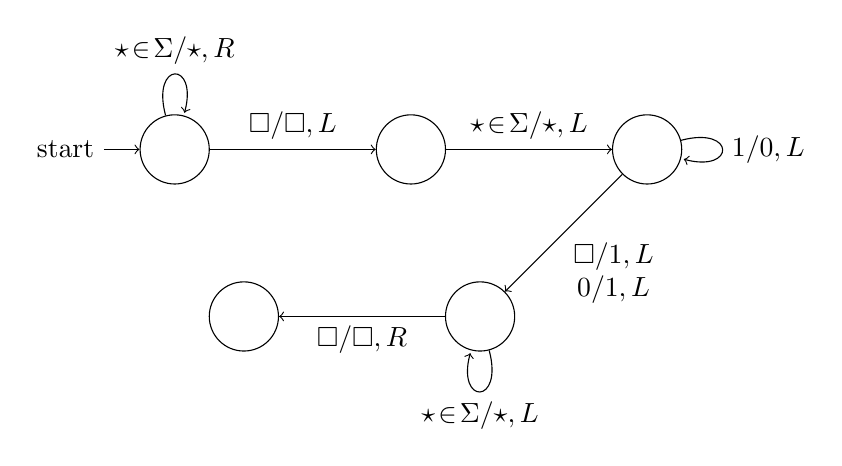
\begin{tikzpicture}[->, auto, node distance=3cm]
	\node[initial,state]   (A) {};
  \node[state]           (B) [right of = A] {};
  \node[state]           (C) [right of = B] {};
  \node[state]           (D) [below left of = C] {};
  \node[state]           (E) [left of = D] {};
  \path (A) edge [loop above] node {$\star\!\in\!\Sigma/\star,R$} (A)
            edge [] node {$\square/\square,L$} (B)
        (B) edge [] node {$\star\!\in\!\Sigma/\star,L$} (C)
        (C) edge [loop right] node {$1/0,L$} (C)
            edge [align=center] node {$\square/1,L$ \\ $0/1,L$ } (D)
        (D) edge [loop below] node {$\star\!\in\!\Sigma/\star,L$} (D)
            edge [] node {$\square/\square,R$} (E);
\end{tikzpicture}

\section{}
\begin{lstlisting}[mathescape]
$x_3$ := 0;
$x_4$ := $x_1$;
$x_5$ := $x_2$;
while($x_4 \neq 0$){
    $x_4$ := $x_4 -1$;
    $x_3$ := $x_3+3$;
}
while($x_5 \neq 0$){
    $x_5$ := $x_5 -1$;
    $x_3$ := $x_3-1$;
}
\end{lstlisting}

\section{}
\begin{lstlisting}[mathescape]
    $x_1 := 600$
L1: print(ab)
    $x_2 := x_2-1$
    if $(x_2\neq0)$ goto L1
    halt
\end{lstlisting}
Die Kolmogorov Komplexität von diesem Programm liegt bei 49 ($<600$, gezählt ohne benötigte Whitespaces). Wir nutzen dabei die Vermutung aus, dass der String wirklich nur aus aneinander gereihten ab's besteht.

\section{}
\begin{enumerate}
	\itemindent3cm
  \item[P:] Ist Array sortiert?
  \item[NP$\backslash$ P:] Hamiltonkreis, BinPacking
  \item[stark NP-vollständig:] Sat, BinPacking
  \item[schwach NP-vollständig:] SubsetSum
\end{enumerate}

\section{}
Der Beweis erfolg durch Reduktion \emph{von} \textsc{HamiltonKreis}.

Der HamiltonKreis ist:
\pbox[t]{.5\textwidth}{
Gegeben ein Graph $G = (V,E)$, gibt es eine Rundtour, die jeden Knoten genau einmal besucht?
}

Mittels der Reduktion müssen wir zeigen, dass \emph{das angekreuzte Problem ein Spezialfall des TSP ist.}

Die Reduktion zur Erstellung einer TSP-Instanz in polynomieller Zeit ist:
\begin{enumerate}
	\item Erstelle einen Graphen $G'$ mit allen Knoten aus $V$ des \emph{HamiltonKreis}es. 
  \item Erstelle für jeden Knoten Kanten zu allen anderen Knoten, die Menge $E'$.
  \item Für jede Kante $e\in E$ setze die Kosten für die korrespondiere Kante $e_1\in E'$ auf 1.
  \item Für jede übrige Kante setze die Kosten auf 2.
  \item Setze $K = |V|$.
\end{enumerate}

Man zeigt dies, indem man die folgenden zwei Beweisschritte nutzt:
\begin{itemize}
	\item Es gibt eine Lösung des \textsc{HamiltonKreis}instanz gdw es eine Lösung des \textsc{TSP} gibt.
  \item Es gibt eine Lösung des \textsc{TSP} gdw es eine Lösung der \textsc{HamiltonKreis}-Instanz gibt.
\end{itemize}

Die zwei Beweisschritte sind:
\begin{itemize}
	\item Es gibt eine Lösung des \textsc{HamiltonKreis}instanz gdw es eine Lösung des \textsc{TSP} gibt: \\
        Wenn das TSP für $K = |V|$ eine Lösung findet, so nutzt diese nur genau Kanten mit den Kosten 1 (und diese nur genau einmal), da sonst die Kosten $K$ überschritten würden. Dadurch wird die Lösung genau zu einem Hamiltonkreis über den Teilgraphen mit den Kanten mit Kosten 1.
  \item Es gibt eine Lösung des \textsc{TSP} gdw es eine Lösung der \textsc{HamiltonKreis}-Instanz gibt. \\
        Wenn die \textsc{HamiltonKreis}-Instanz eine Lösung hat, dann gibt es für $K$ eine Lösung der TSP Instanz.
\end{itemize}

\end{document}